\section*{Chapter 3: Design and Implementation}
\phantomsection \setcounter{section}{3} \setcounter{subsection}{0}
\addcontentsline{toc}{section}{\textit{Chapter 3: Design and Implementation}}

This chapter describes the design and implementation of \texttt{linux-mcp}, a kernel-assisted control plane for LLM tool invocation on Linux.
The central design decision is deliberately narrow in scope yet consequential in effect: tool execution is confined to user space, while admission control and approval state are delegated to a loadable kernel module.

The fundamental limitation of a wholly user-space tool path is not inherent insecurity per se, but rather the conflation of policy, state, and execution within a single trust domain.
In typical MCP-style architectures, the same process that parses tool metadata also decides whether a call may proceed, maintains approval state, and forwards the request to the tool~\cite{mickens2019nightwatch}.
This is convenient to construct, but it means that a compromised or misbehaving mediator can influence every stage of the invocation path.
\texttt{linux-mcp} addresses this by decoupling semantic handling from enforcement: \texttt{mcpd} retains responsibility for manifest parsing, schema validation, session management, and tool routing, while
\texttt{kernel\_mcp} owns registry state, arbitrates invocation requests, manages approval ticket lifecycles, and surfaces the authoritative control-plane state via \texttt{sysfs}.

It is important to state the trust model precisely.
\texttt{mcpd} remains a fully trusted component: it populates the kernel's tool and agent registries, computes all semantic hashes, and derives the binding credentials used for identity verification.
The kernel does not independently re-derive these values from raw sources; it enforces what \texttt{mcpd} has asserted.
What the kernel \emph{does} provide is a stronger enforcement domain for the state that \texttt{mcpd} has established: registry entries, approval tickets, binding checks, and invocation lifecycle transitions are held in kernel space, protected by \texttt{CAP\_NET\_ADMIN} access control on all registry-mutating Netlink commands, and remain inspectable independently of the daemon's process lifetime.
This is not a TCB reduction---\texttt{mcpd} is still trusted---but a \emph{TCB partitioning}: state that benefits from durability, independent observability, and protection from unprivileged interference is held in the kernel, while state that requires semantic flexibility remains in the daemon.



\subsection{Design Goals}

The design is oriented around three concerns that arise from the problem of mediating LLM tool invocations in a trustworthy way.

The foremost requirement is that admission control must not reduce to a user-space daemon unilaterally deciding whether to forward a request.
The admissibility of a tool invocation is determined solely by explicit kernel-resident state: the registration status of the requesting agent, the presence of the target tool in the registry, and the consistency of its semantic identity with the registered manifest.
Anchoring this decision in the kernel ensures it cannot be silently circumvented by tampering with the daemon or by injecting a forged request that the daemon would otherwise accept~\cite{narayan2020shreds}.
This aligns with observations from modern container and system security studies, where enforcing security boundaries outside application logic significantly reduces the attack surface~\cite{xu2021container}.

At the same time, the system must remain compatible with ordinary user-space tools.
Requiring tool authors to expose kernel interfaces or write kernel-facing code would render the system impractical to deploy and would break compatibility with existing tool ecosystems.
In \texttt{linux-mcp}, a tool is simply a resident user-space service bound to a Unix domain socket under \texttt{/tmp/linux-mcp-apps/}---receiving a structured request payload and returning a structured result---with no kernel-facing obligations imposed on tool authors.

The third concern is observability.
Admission, approval, and completion events must not be confined to transient entries in a daemon's in-memory state or application-level logs; they should
be queryable through the kernel's own interfaces, independently of whether \texttt{mcpd} is currently running.
This property is particularly relevant in the context of daemon failure: if \texttt{mcpd} crashes, the kernel-held state should remain inspectable and recoverable without relying on any daemon-side representation.

These goals impose an explicit scope boundary on the design.
\texttt{linux-mcp} does not attempt to verify tool semantics at runtime, enforce a general policy language, or address every attack surface in LLM-based systems.
What it changes is specifically where admission decisions are made and where approval state is maintained.



\subsection{System Architecture}

\begin{figure}[t]
\centering
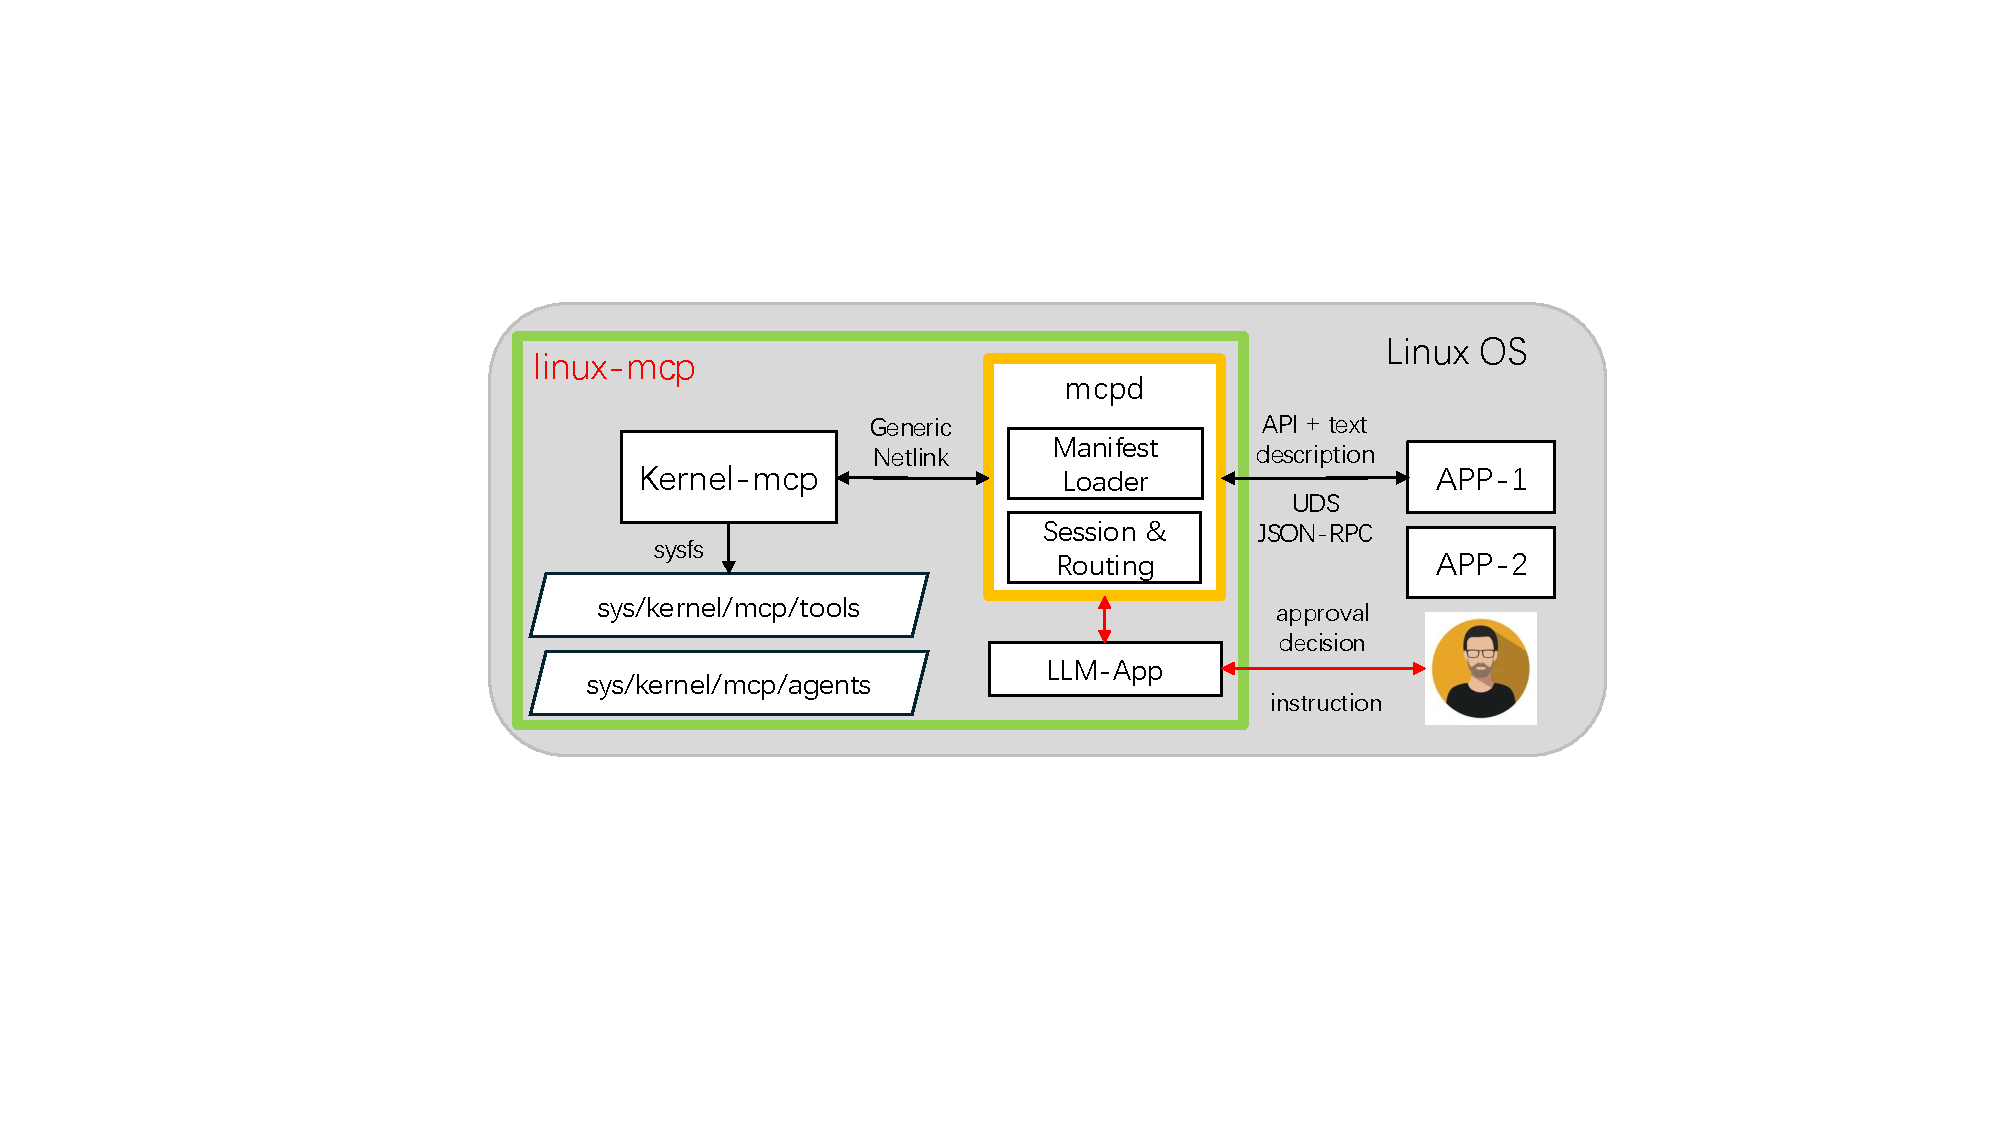
\includegraphics[width=\linewidth,trim=8cm 6cm 6.4cm 4.5cm,clip]{figures/linux-mcp-overview.pdf}
\caption{Overall architecture of \texttt{linux-mcp}.}
\label{fig:linux-mcp-overview}
\end{figure}

The overall architecture of \texttt{linux-mcp}, shown in
Figure~\ref{fig:linux-mcp-overview}, comprises four components.

\texttt{llm-app} is the user-facing client.
It queries \texttt{mcpd} for the tool catalog, constructs invocation payloads from tool schemas, and submits requests.
The client has no direct interaction with the kernel module; all control-plane operations are mediated through \texttt{mcpd}.

\texttt{mcpd} is the user-space gateway and the semantic front-end of the control plane.
It is responsible for loading and validating tool manifests, computing manifest-derived semantic hashes, managing sessions, exposing catalog APIs (\texttt{list\_apps}, \texttt{list\_tools}), communicating with the kernel over Generic Netlink, and forwarding admitted requests to tool services over Unix domain sockets (UDS).
As the sole component with visibility into both tool semantics and runtime transport endpoints, \texttt{mcpd} is correspondingly the only component requiring modification when manifests change or endpoints are reconfigured.

\texttt{kernel\_mcp} is a loadable kernel module implementing the
\texttt{KERNEL\_MCP} Generic Netlink family.
It maintains the tool and agent registries, arbitrates invocation requests, manages approval ticket lifecycles, and exports per-tool and per-agent state through \texttt{sysfs} under \texttt{/sys/kernel/mcp/}.
It neither parses manifests nor executes tools nor implements a general policy language; its sole responsibility is enforcing the compact set of invariants required for admission control.

\texttt{tool-app} is the execution side: a collection of resident user-space services, each bound to a Unix domain socket.
When a request is admitted, \texttt{mcpd} forwards the payload to the appropriate tool service, which executes in an ordinary user-space environment and returns its result to \texttt{mcpd}, which then reports completion back to the kernel.

To clarify the separation of responsibilities across layers,
Table~\ref{tab:architecture_layers} summarises each component together with its intended scope and explicitly excluded functionality.

\begin{table}[t]
\centering
\small
\begin{spacing}{1.1}
\begin{tabular}{l p{3cm} p{4.8cm} p{4.5cm}}
\toprule
\textbf{Layer} & \textbf{Component} & \textbf{Main responsibility} & \textbf{Intentionally excluded} \\
\midrule

Client layer 
& \texttt{llm-app} CLI/GUI
& Discover tools, plan usage, open sessions, submit requests, handle approvals
& Direct tool access, direct kernel communication \\

Gateway layer 
& \texttt{mcpd}
& Load manifests, compute semantic hash, validate payloads, bind sessions, route requests, communicate with kernel
& Durable governance state independent of process lifetime \\

Kernel layer 
& \texttt{kernel\_mcp}
& Maintain registries, perform admission decisions, manage approval tickets, expose \texttt{sysfs} state
& JSON parsing, tool execution, LLM-specific logic \\

Execution layer 
& Tool services
& Execute application logic and return structured results
& Global policy enforcement \\

\bottomrule
\end{tabular}
\end{spacing}
\caption{Concrete layers in \texttt{linux-mcp}.}
\label{tab:architecture_layers}
\end{table}



\subsection{Control-Plane Workflow}

\begin{figure}[t]
\centering
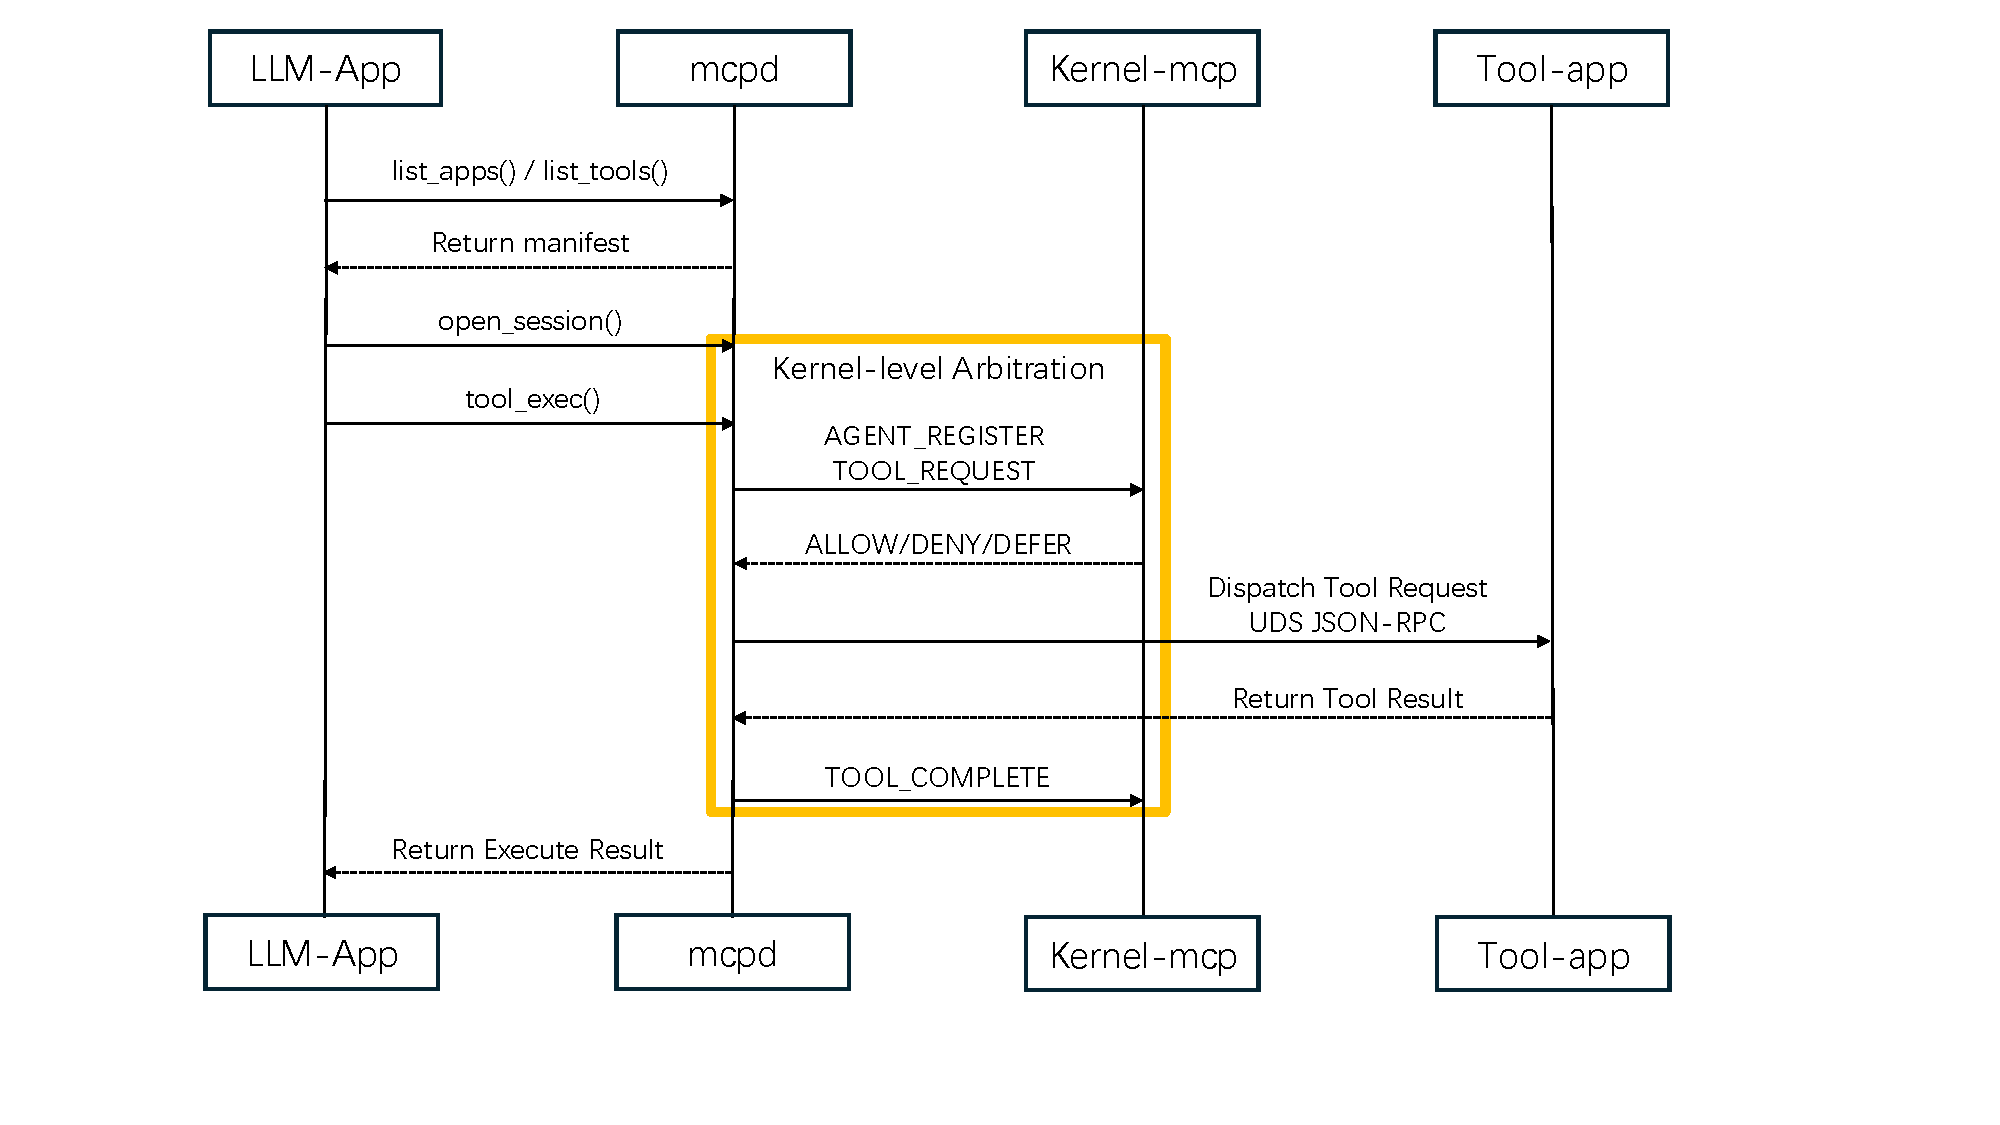
\includegraphics[width=\linewidth,trim=1cm 1.5cm 2cm 0cm,clip]{figures/linux-mcp-workload.pdf}
\caption{Invocation lifecycle in \texttt{linux-mcp}.}
\label{fig:chapter3-lifecycle}
\end{figure}

The end-to-end request path is:
\[
\texttt{llm-app} \to \texttt{mcpd} \to \texttt{kernel\_mcp} \to
\texttt{mcpd} \to \texttt{tool-app} \to \texttt{mcpd} \to \texttt{llm-app}
\]
Figure~\ref{fig:chapter3-lifecycle} illustrates this path as a sequence diagram.
A request originates in \texttt{llm-app}, which first issues a catalog query that \texttt{mcpd} satisfies from its manifest-derived in-memory state.
The kernel occupies this path not as a passive observer but as the active arbitration point: \texttt{mcpd} cannot forward a request to a tool without first obtaining an \texttt{ALLOW} decision from the kernel, and it cannot
close an invocation without reporting \texttt{TOOL\_COMPLETE} back through the same channel.
This renders admission and completion as explicit, kernel-visible state transitions rather than implicit control-flow decisions internal to the daemon.

The catalog response includes the tool name, input schema, description, risk tags, examples, and other metadata.
The client uses this information to construct a structured invocation payload and submits it as a \texttt{tool:exec} call to \texttt{mcpd}.

Upon receiving the request, \texttt{mcpd} performs a series of user-space checks: it resolves the active session, validates the payload against the declared input schema, identifies the target tool, and retrieves the semantic hash associated with that tool from its manifest-derived state.
Only upon successful completion of these checks does \texttt{mcpd} issue a
\texttt{TOOL\_REQUEST} to the kernel, supplying the agent identifier, tool identifier, and semantic hash as parameters.

The kernel module then performs arbitration.
It verifies that the requesting agent is in the agent registry, that the target tool is in the tool registry, and that the semantic hash in the request matches the hash recorded at registration time.
Based on these checks and the tool’s policy, the kernel returns a decision that determines whether the request can proceed immediately, must be rejected, or requires further approval.
The detailed semantics of these decisions are described in Section~\ref{fig:chapter3-approval}.

Depending on the kernel’s decision, \texttt{mcpd} either forwards the request to the tool service, terminates the invocation with an error, or transitions the request into a pending state awaiting external approval.
After the tool service returns a result, \texttt{mcpd} issues \texttt{TOOL\_COMPLETE} to the kernel, closing the invocation lifecycle in the control plane’s view.

This workflow has a concrete security consequence: the kernel both opens and closes every invocation.
An invocation that never reaches \texttt{TOOL\_COMPLETE}---whether due to daemon failure or tool timeout---persists as an open entry in kernel state and remains inspectable via \texttt{sysfs}.
This contrasts with a purely user-space design, where the lifecycle of a request is only as durable as the daemon's own in-memory representation.



\subsection{Manifest Semantics and Tool Identity}

A control plane that arbitrates based on tool identity requires a stable definition of what makes two tool registrations refer to the same logical tool.
Tying identity to transport details---socket paths, port numbers, endpoint URIs---causes routine operational changes to generate spurious re-registration events and demands policy reconciliation on every redeployment.
If identity is too coarse, the system cannot distinguish a tool that has been semantically modified from one that has simply been redeployed at a different address.

\texttt{linux-mcp} resolves this by separating semantic identity from transport location.
Each tool is described by a JSON manifest containing logical attributes: tool identifier, tool name, application identifier, application name, risk tags, description, input schema, examples, path semantics, and approval policy.
These fields describe what the tool is intended to do, not where it runs.
\texttt{mcpd} canonicalizes the semantically relevant field subset into a stable JSON representation and computes the full 256-bit SHA-256 digest over it, represented as a 64-character hexadecimal string.
The full digest is used without truncation: a truncated prefix (e.g., 8 hex characters, 32 bits) would allow collisions by the birthday bound after approximately $2^{16}$ tool registrations, which is not a large number in a production system spanning many applications.
Crucially, the Unix domain socket endpoint is excluded from the hash computation.
A tool may therefore be redeployed to a new socket path without changing its logical identity, provided the semantic fields in the manifest remain unchanged.
Conversely, any modification to a semantically significant field---the input schema, risk tags, description, approval policy, or path semantics---produces a different 256-bit digest, which the kernel detects as a mismatch upon the next \texttt{TOOL\_REQUEST}.

This separation matters for admission control because the kernel and the daemon can only meaningfully agree on whether a request is legitimate if they share a common notion of tool identity.
The semantic hash is the concrete artefact that makes this agreement possible: it is computed in user space but verified in kernel space, so the daemon cannot substitute a different tool without producing a detectable hash mismatch.




\subsection{Session Management and Approval Binding}

Approval is one of the more subtle aspects of the control path to get right.
Deferring and resolving a request is straightforward; ensuring that an approval applies to the exact same session, requester, and operation requires explicit binding and precise state tracking.

In \texttt{linux-mcp}, each session maintained by \texttt{mcpd} is bound to the real peer credentials of its Unix domain socket connection \cite{stevens2013unix}.
From these credentials, the daemon derives a \emph{binding hash} and a
\emph{binding epoch}.
When a request enters the \texttt{DEFER} state, the kernel creates an approval ticket and associates it with this binding context.
Upon receiving an \texttt{APPROVAL\_DECIDE} message, the kernel verifies that the binding context stored in the ticket still matches the current session state before permitting the deferred request to proceed.

This binding mechanism ensures that approvals cannot be replayed across sessions or misdirected to structurally similar but distinct requests.
More importantly, it guarantees that the system state validated at deferral time is identical to the state at execution time, eliminating time-of-check-to-time-of-use (TOCTOU) inconsistencies \cite{bishop2003computer}.

Beyond basic ticket binding, the implementation reveals a more nuanced structure: \texttt{linux-mcp} employs \emph{two layers of arbitration} and supports \emph{two distinct approval paths}.

\textbf{(1) Kernel-mediated approval path (DEFER ticket flow).}
In this path, the kernel acts as the authoritative control-plane arbiter.
A \texttt{TOOL\_REQUEST} may result in:
\begin{itemize}
    \item \texttt{ALLOW}: the request proceeds directly to execution
    \item \texttt{DENY}: the request is rejected immediately
    \item \texttt{DEFER}: the kernel suspends execution and issues an approval ticket
\end{itemize}
When a request is deferred, \texttt{mcpd} records the pending operation and returns the ticket identifier to the client.
After user approval, \texttt{mcpd} first sends \texttt{APPROVAL\_DECIDE} to the kernel to update the ticket state, and only then replays the original request with the associated ticket.
The kernel consumes the ticket during the second \texttt{TOOL\_REQUEST} and allows execution to proceed.

\textbf{(2) User-space policy path (local approval).}
Separately, \texttt{linux-mcp} supports a local approval mechanism driven by \texttt{approval\_policy} in the manifest.
In this case, \texttt{llm-app} may prompt the user for confirmation \emph{before} issuing a request to \texttt{mcpd}.
If denied, the request is rejected locally without entering the kernel arbitration path, and no approval ticket is created.
This separation allows low-cost semantic checks to be handled in user space while reserving kernel mediation for high-risk operations.

Figure~\ref{fig:chapter3-approval} illustrates the complete invocation lifecycle, spanning both user space and kernel space.
A request originates in \texttt{llm-app}, which establishes a session and sends a \texttt{TOOL\_REQUEST} via \texttt{mcpd}.
The kernel performs arbitration and returns \texttt{ALLOW}, \texttt{DENY}, or \texttt{DEFER}.

In the \texttt{DEFER} case, the request transitions into a \emph{pending state}, and the system waits for an explicit user decision.
Only after the user approves the request and \texttt{APPROVAL\_DECIDE} is processed by the kernel does the request re-enter the execution path and reach the tool service.
The critical ordering, as shown in Figure~\ref{fig:chapter3-approval}, is that approval resolution occurs \emph{before} tool execution, ensuring that no deferred request can bypass the approval gate and that every execution corresponds to an explicitly validated ticket.

This mechanism reflects a key design principle in \texttt{linux-mcp}.
User space is responsible for interpreting semantics---including request structure, tool schemas, and policy hints---while the kernel enforces \emph{minimal, stable invariants} over state transitions.
The kernel does not need to understand the full meaning of a request; it only needs to ensure that: the binding context is preserved, the approval ticket is valid and unconsumed, and the state transition (\texttt{DEFER} $\rightarrow$ \texttt{ALLOW}) is explicitly authorised.
By constraining the trusted computing base to these minimal, stable invariants \cite{saltzer1975protection}, \texttt{linux-mcp} achieves meaningful safety guarantees without embedding high-level application semantics in kernel space.

\begin{figure}[t]
\centering
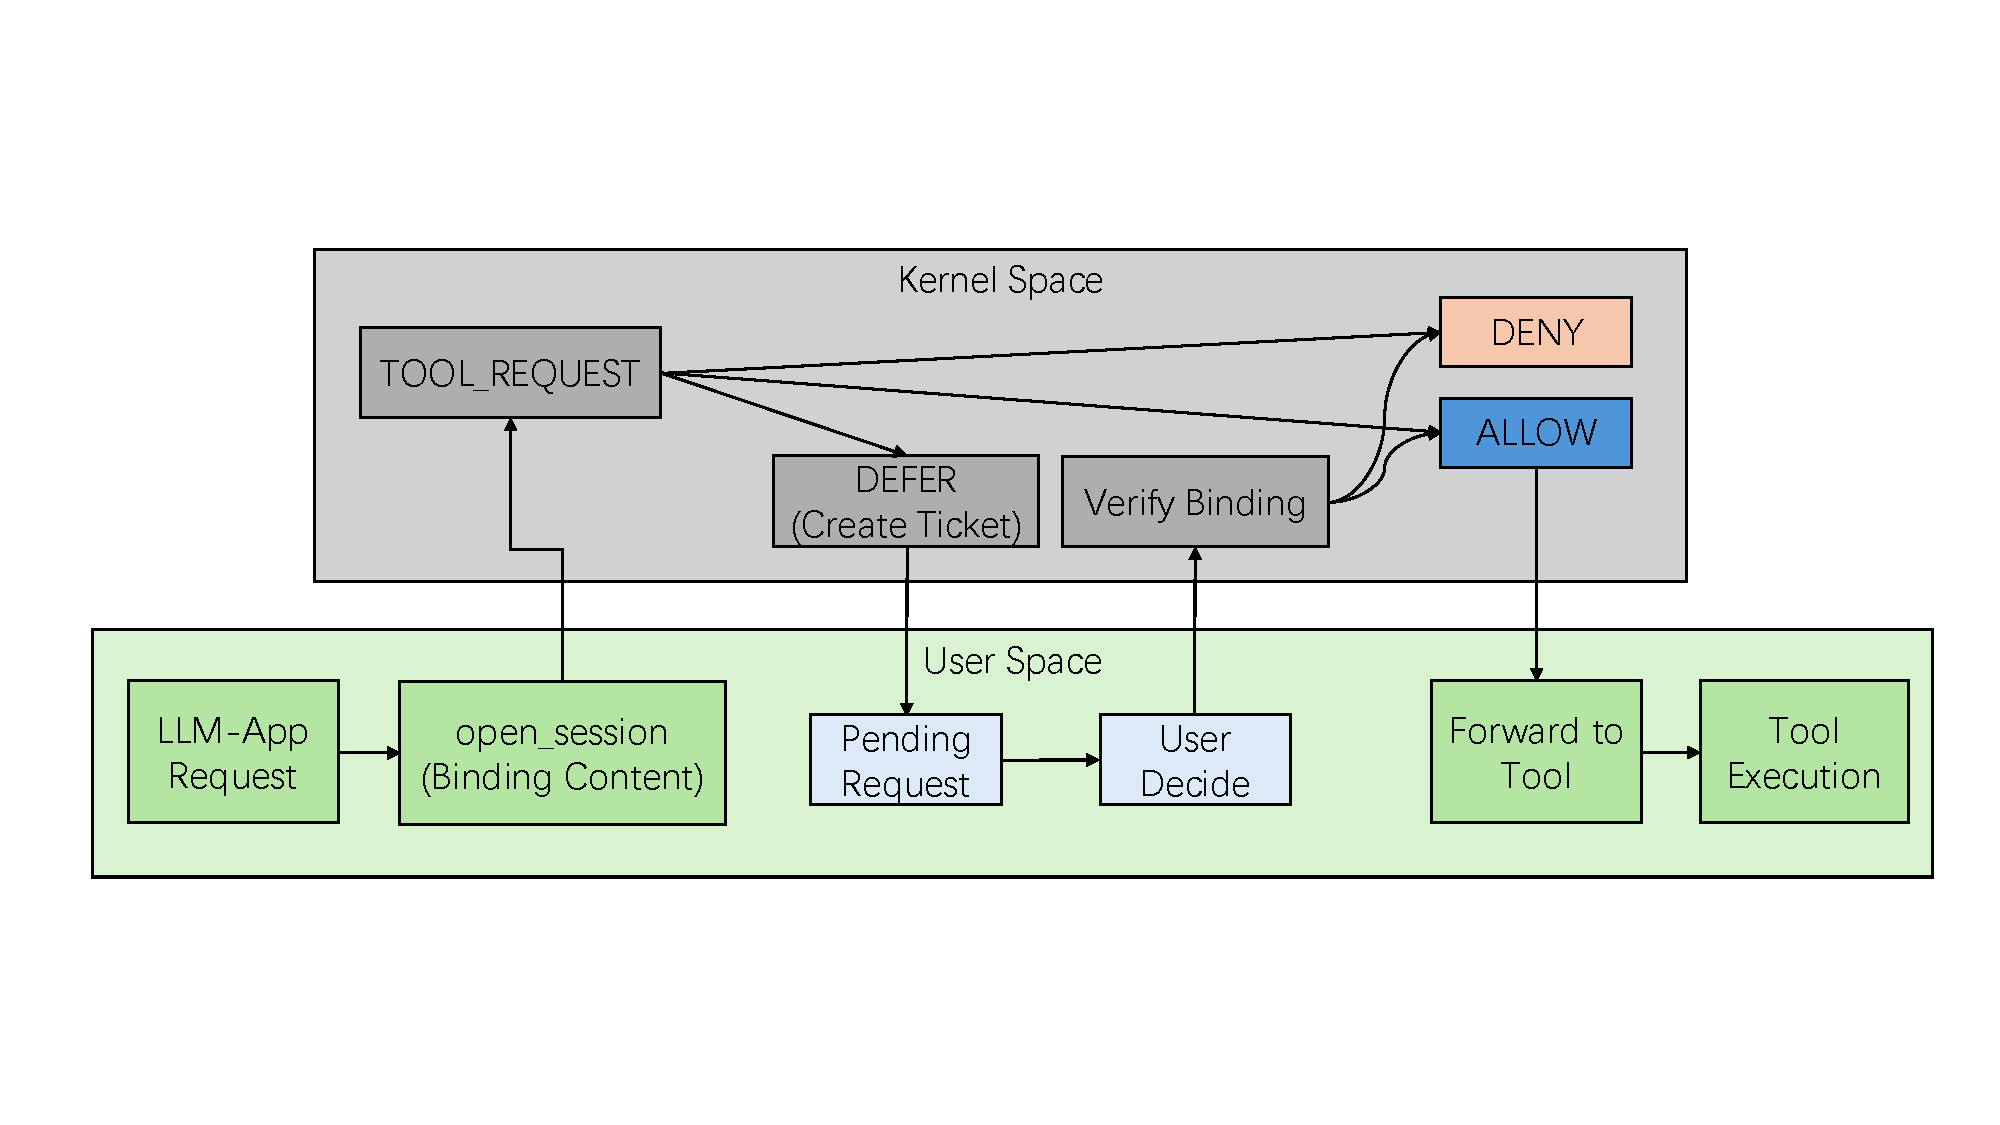
\includegraphics[width=\linewidth,trim=0.5cm 2cm 0cm 2cm,clip]{figures/linux-mcp-approval.pdf}
\caption{Invocation lifecycle in \texttt{linux-mcp}.}
\label{fig:chapter3-approval}
\end{figure}



\subsection{Kernel Module Design}

The kernel module is implemented as a Generic Netlink family named \texttt{KERNEL\_MCP}.
The command set covers the full invocation lifecycle: \texttt{TOOL\_REGISTER}, \texttt{AGENT\_REGISTER}, \texttt{TOOL\_REQUEST}, \texttt{TOOL\_DECISION}, \texttt{TOOL\_COMPLETE}, \texttt{APPROVAL\_DECIDE}, \texttt{RESET\_TOOLS}, and \texttt{LIST\_TOOLS}.
Generic Netlink was preferred over alternatives such as \texttt{ioctl} or character devices for three reasons: it provides a naturally structured message format, supports dump-style enumeration for registry introspection, and yields a self-describing kernel interface well suited to a research prototype \cite{netlink2026}.

Internally, the module maintains two registries.
The tool registry maps tool identifiers to their manifest-derived semantic hashes and associated metadata.
The agent registry records the identifiers of entities permitted to submit requests through the control plane.
Approval tickets are heap-allocated kernel objects with explicit lifecycle fields tracking whether a ticket has been decided, approved, consumed, or expired.

The arbitration logic is deliberately narrow.
For a \texttt{TOOL\_REQUEST} to be admitted, three conditions must all hold: the submitting agent must appear in the agent registry, the target tool must appear in the tool registry, and the semantic hash provided by \texttt{mcpd} must match the hash recorded at tool registration.
If the tool's manifest marks it as requiring explicit approval, the request is deferred rather than immediately allowed.
The aim of this prototype is not to embed a rich policy language in the kernel, but to demonstrate that the kernel can authoritatively own the specific state transitions on which safe admission depends---transitions that cannot be bypassed from user space.

The module also exports state through \texttt{sysfs}.
Under \texttt{/sys/kernel/mcp/tools/}, each tool has a directory containing its name, hash, and related metadata.
Under \texttt{/sys/kernel/mcp/agents/}, per-agent entries record counters such as \texttt{allow}, \texttt{defer}, \texttt{completed\_ok}, and \texttt{last\_exec\_ms}, together with a human-readable \texttt{last\_reason} field.
This observability is valuable both during development and during evaluation: the experimenter can verify which tools are registered, confirm which hashes the kernel regards as authoritative, and inspect the kernel's view of agent activity independently of any daemon-side logs.



\subsection{Daemon Implementation}

While the kernel enforces the critical state transitions, \texttt{mcpd} is where most of the system's substantive work takes place.
Its implementation is organised around four responsibilities: manifest processing, session management, kernel communication, and tool routing.

The manifest loader is the semantic entry point of the system.
It parses tool description files from \texttt{tool-app/manifests/}, enforces transport constraints (only \texttt{uds\_rpc} transport is currently supported, and endpoints must reside under \texttt{/tmp/linux-mcp-apps/}), and computes semantic hashes.
The manifest-derived catalog also serves as the authoritative source for what \texttt{llm-app} sees when it queries \texttt{list\_apps} or \texttt{list\_tools}.

The session store maintains active connections together with their peer-derived binding information and any pending approval context.
This gives the daemon sufficient information to associate incoming approval decisions with the correct deferred request, without requiring the kernel to store full session semantics.
The binding information---derived from Unix domain socket peer
credentials---is what gets embedded in approval tickets.

The Netlink client provides a persistent communication channel to the kernel module.
A dedicated, long-lived socket is maintained rather than opening a new connection per request; this keeps the control path measurable and avoids repeated socket-setup overhead.
Per-stage timing---covering session lookup, kernel arbitration, tool execution, and end-to-end latency---can optionally be recorded for each invocation, which is useful for separating control-plane overhead from tool-side processing time during evaluation.

The server-facing side of \texttt{mcpd} handles two distinct roles: it exposes the catalog and invocation interfaces consumed by \texttt{llm-app}, and it forwards admitted requests to the appropriate \texttt{tool-app} service via the same Unix domain socket transport used on the tool side.



\subsection{Tool-Side RPC and Execution Model}

The tool-side protocol is intentionally simple.
Each tool service is a resident process bound to a Unix domain socket, receiving framed JSON messages with a 4-byte big-endian length prefix.
The length-prefixed framing eliminates stream-parsing ambiguity and keeps the transport entirely independent of the kernel control plane---tool authors need not be aware of Generic Netlink or any kernel interface.

This simplicity has practical consequences beyond compatibility.
Because the tool executes in an ordinary user-space environment with no kernel-facing obligations, the boundary between admission and execution is unambiguous: the kernel decides whether a request may proceed; everything about what the request means and how it is executed remains in user space.
Failure handling follows naturally from this separation.
If a tool crashes, times out, or returns an error, \texttt{mcpd} handles the event in user space and reflects it back to the kernel through \texttt{TOOL\_COMPLETE}, marking the invocation lifecycle as closed.
The kernel requires no visibility into how the tool failed internally.



\subsection{State Reconciliation and Recovery}

A design that splits state across the kernel and a user-space daemon must handle the case where the two sides diverge.
\texttt{mcpd} may restart---intentionally during development, or unintentionally following a crash---while the kernel module remains loaded with its existing registry state.
If manifests change between a crash and a restart, the tool hashes registered in the kernel will no longer match the hashes derived from the current manifest files, and subsequent \texttt{TOOL\_REQUEST} messages will be denied with
\texttt{hash\_mismatch}.

\texttt{linux-mcp} addresses this with a reconciliation path.
On startup, \texttt{mcpd} issues a \texttt{RESET\_TOOLS} command to clear the kernel-side tool registry, then re-registers the full set of tools from the current manifest state.
This is a deliberately conservative strategy: the system unconditionally rebuilds state from the manifest source of truth rather than attempting to assess whether residual kernel state remains valid.
This trade-off is appropriate for a research prototype, where state correctness and auditability take precedence over minimising re-registration overhead.

It is worth noting what kernel-held approval state provides in this context.
After a daemon crash, session state is lost---the binding context for in-progress sessions no longer exists in user space.
However, approval tickets recorded in the kernel before the crash remain visible through \texttt{sysfs}, enabling post-mortem inspection even in the absence of a running daemon.
This behaviour is confirmed in the experimental evaluation: after an induced daemon failure, approval state was preserved in the kernel-mediated path while the user-space-only baseline lost it entirely.



\subsection{Rationale for the Kernel--User-Space Split}

The architecture of \texttt{linux-mcp} is positioned between two degenerate extremes.
A purely user-space architecture consolidates policy, state, and execution within a single trust domain---easy to construct, but equally easy to subvert.
Conversely, a kernel-heavy design that relocates manifest parsing and tool execution into kernel space would be neither safe nor practically deployable: JSON parsing in kernel space introduces an unnecessarily large attack surface, and tool integration belongs in an environment that supports flexible language runtimes and evolving schemas.

The split adopted here avoids both extremes.
User space retains everything that benefits from flexibility: manifest semantics, payload validation, session logic, and tool execution.
The kernel retains the smaller, more stable set of operations that benefit from stronger authority and independently inspectable state: which tools and agents are registered, whether a given request may advance, whether an approval ticket is valid and unconsumed, and whether an invocation has been formally closed.
This constitutes the central implementation claim of the system, and it is precisely what the evaluation presented in the following chapter is designed to validate.

\paragraph{Design alternatives considered.}

Three kernel-interface alternatives were considered before settling on a Generic Netlink family.

\textbf{Linux Security Module (LSM) hooks.}
LSM hooks attach to VFS and socket operations at fixed kernel hook points~\cite{lsm2026}.
They can enforce access control over file opens, socket sends, and process creation, but they cannot natively express the notion of ``this Netlink message carries a valid semantic hash for this registered tool.''
Maintaining a dynamically populated, per-tool hash registry at LSM hook granularity would require storing tool state in LSM blob storage and correlating it with Netlink message content at hook time---a design that is both complex and fragile, since LSM hooks fire at the system-call boundary rather than at the application-protocol boundary where tool identity is meaningful.

\textbf{eBPF programs attached to the Netlink socket.}
An eBPF program can filter socket operations and enforce byte-level policies with very low overhead~\cite{seccomp2026}.
However, the eBPF verifier's memory and loop restrictions make it impractical to maintain a dynamic hash registry inside a BPF map and perform variable-length string comparisons at hook time without significant complexity.
More importantly, eBPF programs cannot issue Netlink replies or manage kernel-side lifecycle state (approval tickets, counters) without a userspace control plane---which reintroduces the dependency on user-space correctness that the design aims to reduce.

\textbf{Capsicum-style capability model.}
A Capsicum-style design~\cite{watson2010capsicum} could scope each tool invocation to a capability derived from the tool's identity, preventing escalation across tool boundaries.
This approach would require tool services to be written against a capability API, violating the design goal of tool-author transparency: existing tool services should require no modification to participate in the control plane.

A Generic Netlink family avoids all three limitations.
It provides a structured, self-describing message format; supports dump-style enumeration for registry introspection; allows the kernel module to maintain full lifecycle state (registries, tickets, counters) without verifier constraints; and imposes no interface requirements on tool authors.
The cost is that it requires a loadable kernel module rather than a policy layer attached to existing hooks---a trade-off that is appropriate for a research prototype but would need careful security review for production use.